\documentclass[../main.tex]{subfiles}
% b = k × λ ÷ sin(α)
%   α = 30°; λ = 530nm
%   -> b = 1500nm

\subsection{Versuchsaufbau}

\begin{figure}[ht]
    \centering
    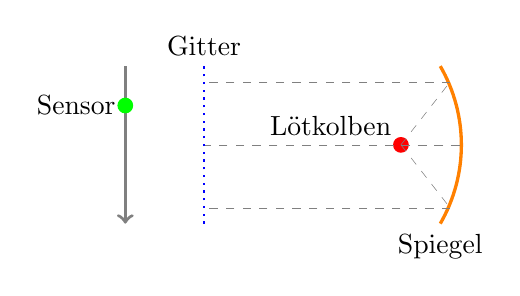
\begin{tikzpicture}
        %\draw[step=1] (-3,-2) grid (4,2);
        
        \draw (3,1)[orange,very thick] arc (30:-30:2cm) node[black,anchor=north] {Spiegel};
        \fill[red] (2.5,0) circle (0.1cm) node[black,anchor=south east] {Lötkolben};
        
        % EM-Strahlungsreflektion
        \draw[gray,dashed,very thin] (2.5,0) -- (3.125,0.8);
        \draw[gray,dashed,very thin] (2.5,0) -- (3.125,-0.8);
        \draw[gray,dashed,very thin] (2.5,0) -- (3.25,0);
        
        \draw[gray,dashed,very thin] (3.125,0.8) -- (0,0.8);
        \draw[gray,dashed,very thin] (3.125,-0.8) -- (0,-0.8);
        \draw[gray,dashed,very thin] (3.25,0) -- (0,0);
        
        \draw[blue,thick,dotted] (0,-1) -- (0,1) node[black,anchor=south] {Gitter};
        
        \draw[very thick,gray,->] (-1,1) -- (-1,-1);
        \fill[green] (-1,0.5) circle (0.1cm) node[black,anchor=east] {Sensor};
    \end{tikzpicture}
    \caption{Aufbau}
    \label{fig:experiment_aufbau}
\end{figure}

% Bilder:
%   - loetkolben
%   - hg-lampe
%   - spiegel
%   - sensor
%   - gitter

\subsection{Ergebnisse}

% Diagramme
% Fehler
